%% AVB-Engage, JAIHC submission version (Journal of Ambient Intelligence and Humanized Computing, journal 12652).
%% Springer Nature sn-jnl template v3.1 (Dec 2024), [pdflatex,iicol,sn-basic]: two columns, author-year references.
%% JAIHC rules: 12 pages including references at submission (14 after revision), abstract 150-250 words, 4-6
%% keywords, at most three heading levels, "Statements and Declarations" before the references, LLM use documented
%% in the Methods, references alphabetized with DOI links. Supplementary material: supplementary.tex, submitted as
%% Online Resource 1 (ESM_1.pdf). Cut from the 22-page long version on 2026-11-03/09; checked against the code and
%% the result files on 2026-11-13 (docs/plan.md Sec. 21).
%% Section pattern follows the two Springer exemplars (J Ambient Intell Humaniz Comput 17:1579-1598, 2026; J Signal
%% Process Syst 97:269-280, 2025); prose follows the FoleyGAN style (Ghose & Prevost, IEEE TMM 2023).
%% Numbers trace to results/fullclip/, results/paper_springer/ and results/paper_jaihc/ (scripts/paper/*.py), except the training sweep and
%% the 9-of-10 audio check of the earlier sweep (results/night/, docs/plan.md Sec. 13.14), the 67.82 threshold oracle (Sec. 19.6), the
%% fusion weight rules (Sec. 19.7.1), the OpenFace timing (Sec. 18.16) and the pre-training stages (Sec. 18.18):
%% results/engagenet_h8_uniform_fullaudio_v96 (CE, 1e-2, 30 ep) -> results/v12_05_* (ordinal, 1e-4, 25 ep) ->
%% results/exp2026/E04_* (ordinal, 5e-5, 8 ep).
%% Follows the Springer Nature template user manual (v3.1): figures are single image files Fig1-Fig3 on the same level
%% as this file (manual Sec. 7.3; Fig3.pdf is compiled from figures/Fig3_source.tex, Fig1/Fig2 are draw.io exports
%% with sources in figures/src/: make_*_drawio.py write the .drawio files at final size, 84/174 mm with 9-pt lettering
%% (FreeSans, a Helvetica clone), Fig1 with the data of one test clip read from the result files, and export_drawio.js
%% exports them), references are in references.bib and formatted by sn-basic.bst (Sec. 8.3), back-matter
%% heads use \bmhead (Sec. 8.1). Not [referee]: JAIHC's own 12-page two-column rule takes precedence (manual Sec. 1).
%% Each figure exists as FigN.pdf and FigN.eps (manual Sec. 7.3: "LaTeX compiler accepts only .eps"); \includegraphics{FigN}
%% has no extension, so pdfLaTeX uses the PDF and latex/dvips the EPS. After changing a PDF, regenerate its EPS with
%% Ghostscript: gs -q -dNOPAUSE -dBATCH -dSAFER -sDEVICE=eps2write -sOutputFile=FigN.eps FigN.pdf

\documentclass[pdflatex,iicol,sn-basic]{sn-jnl}

\usepackage{graphicx}
\usepackage{multirow}
\usepackage{amsmath,amssymb,amsfonts}
\usepackage{xcolor}
\usepackage{booktabs}
\usepackage{algorithm}
\usepackage{algorithmicx}
\usepackage{algpseudocode}

% Model name used throughout. Change it here only.
\newcommand{\ournet}{AVB-Engage}

\raggedbottom

\begin{document}

\title[AVB-Engage: audio-visual and facial-behavior fusion for engagement recognition]{AVB-Engage: Audio-Visual and Facial-Behavior Fusion for Ordinal Student Engagement Recognition}

% Title block filled 2026-11-14: Yuvraj Gupta is the corresponding author (*); ORCIDs go into the submission form.
\author*[1]{\fnm{Yuvraj} \sur{Gupta}}\email{ygupta@sfsu.edu}
\author[1]{\fnm{Sanchita} \sur{Ghose}}\email{sanchitaghose@sfsu.edu}
\affil*[1]{\orgdiv{Department of Computer Science}, \orgname{San Francisco State University}, \orgaddress{\street{1600 Holloway Avenue}, \city{San Francisco}, \state{CA} \postcode{94132}, \country{USA}}}

\abstract{Automatic engagement recognition estimates from a webcam recording how engaged a student is during online learning. The task is harder than its four classes suggest: the engagement levels are ordered and imbalanced, the two middle levels look alike within a ten-second clip, and the audio track of a student watching an educational video carries a weak signal, so recent methods read the visual stream only. In this paper, we present \ournet{} (audio, video and behavior), which fuses three sources of evidence. An audio-visual cross-attention network lets the face frames and the log-mel spectrogram attend to each other after the audio steps are pooled onto the video frames, and two models built on segment statistics of OpenFace action units, gaze and head pose read the facial behavior of the same clip. The class probabilities of the three models are averaged and decoded through the expected engagement level with thresholds fitted on the validation split, so that the order of the levels is used at prediction time. We evaluated \ournet{} on the official EngageNet test split over three training seeds. Adding audio to video raises top-1 accuracy in seven of nine trained networks, decoding through the expected level adds 1.99 points over argmax decoding on identical weights, and averaging the network with the two behavior models adds about four points more because the models make different errors. \ournet{} reaches 70.29\% top-1 accuracy and a mean absolute error of 0.401 levels, against 67.61\% for the best published test-split result.}


\keywords{Student engagement recognition, Audio-visual fusion, Cross-attention, Facial action units, Ordinal classification, Online learning}

\maketitle

\section{Introduction}\label{sec:intro}

An instructor who teaches online sees each student only as a tile on a screen, and automatic engagement recognition aims to tell from each student's webcam recording who was disengaged \citep{qarbal2025review,mandia2023review}. A ten-second clip offers three kinds of evidence: the face frames, the audio track, and the facial behavior of the student, such as action units, gaze and head pose. The clip is labeled with one of four ordered levels, from \emph{not engaged} to \emph{highly engaged}. The order matters, since calling a highly engaged student \emph{not engaged} is a larger error than calling the student \emph{engaged}, and the levels are imbalanced: half of the test clips are \emph{highly engaged}, and the two middle levels are rare and visually similar, so they attract most of the errors. Recent methods read the visual stream only \citep{singh2023engagenet,vedernikov2024tcct,abedi2024stgcn,vedernikov2026priornet,augusma2026vemd}, because the audio of a student watching an educational video is noisy, often absent, and rarely contains speech.

In this paper, we propose \ournet{} (audio, video and behavior), which predicts the engagement level of a clip from all three sources of evidence (Fig.~\ref{fig:overview}). An audio-visual network (A) encodes the face frames with an EfficientFace backbone \citep{zhao2021efficientface} and the log-mel spectrogram with a convolutional encoder, and lets the two streams attend to each other through three cross-attention stages, following audio-visual emotion recognition \citep{venkatraman2025avtca}; the audio steps of each clip are pooled onto its video frames beforehand, so that each visual token has one audio token for the same time span. Two models (B), a gradient-boosting classifier and a small Transformer encoder, read the OpenFace descriptor of the same clip as segment statistics, the tokenization of the strongest published baseline \citep{singh2023engagenet}. A late fusion stage (C) averages the three probability vectors and reads the result as a position on the ordered scale, which is then cut at thresholds fitted on the validation split. The behavior models are kept separate from the network because models trained on different inputs with different learners make different errors.

\begin{figure}[t]
\centering
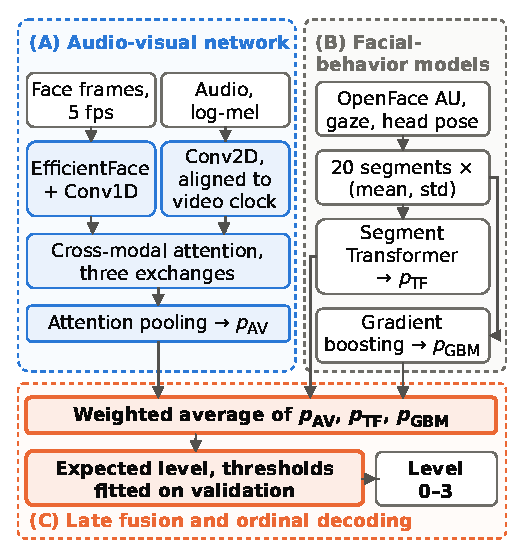
\includegraphics[width=\columnwidth]{Fig1}
\caption{Overview of \ournet, shown on a test clip whose true level is \emph{engaged} (models of the first seed). (A) The audio-visual network reads the face frames, drawn here schematically, and the log-mel spectrogram; (B) two models read segment statistics of the OpenFace descriptor (three of its 22 channels shown); (C) the class probabilities of the three models are averaged with fixed weights, and the expected level $\mu$ of the average is cut at the thresholds $\tau_1$--$\tau_3$ fitted on the validation split}
\label{fig:overview}
\end{figure}

The main contributions of this paper are as follows:
\begin{enumerate}
\item We present \ournet, an audio-visual cross-attention model for engagement recognition that uses the audio track alongside the facial and behavioral cues read by recent methods. Audio alone does not exceed the majority-class predictor, yet adding it to video raises top-1 accuracy in most of the trained networks we tested.
\item We measure, on identical trained weights, how much the decoding rule changes accuracy on the ordered scale: decoding through the expected level changes top-1 accuracy more than any training change we tested.
\item We show that facial-behavior descriptors help when they are summarized by segment statistics in separate models and averaged with the network, which exceeds the best published test-split result, whereas the same descriptors learned inside the network change no metric; the gain traces to the different errors of the three models.
\end{enumerate}

\section{Related work}\label{sec:related}

Engagement recognition asks a model to judge from a recording what an annotator judges from a learner's gaze, expression and posture. The main datasets are DAiSEE \citep{gupta2016daisee}, EngageNet \citep{singh2023engagenet}, which labels ten-second clips of students watching educational videos with four ordered levels and has the most participants, and CMOSE \citep{wu2024cmose}, which provides audio as well as video. On EngageNet, the released baselines read OpenFace gaze, head-pose and action-unit statistics or MARLIN video features \citep{singh2023engagenet}; later methods read head-pose signals in the two-stream TCCT-Net \citep{vedernikov2024tcct}, facial landmarks in an ordinal spatial-temporal graph network \citep{abedi2024stgcn}, the face video in PriorNet \citep{vedernikov2026priornet} and in the variational encoder VE-MD, which has an audio branch for other datasets but uses video only for engagement \citep{augusma2026vemd}, or facial features, key points and physiological signals estimated from the video in GLP-fusion \citep{qin2026glpfusion}. Gradient boosting on action units has estimated the mental states of learners in a tutoring system \citep{wang2026shap} and reached higher accuracy than the deep networks trained alongside it on two engagement datasets \citep{das2025optimizing}. All of these methods read the visual stream only. The closest result to our use of audio comes from CMOSE: adding audio features to its visual features raises accuracy only slightly over all test segments, but clearly on the quarter of segments that contain speech \citep{wu2024cmose}.

Audio-visual fusion has been developed mainly for emotion recognition, where the voice and the face express the same affective state; AVT-CA \citep{venkatraman2025avtca} fuses the two streams with transformer cross-attention, in which each modality attends to the other. A student watching an educational video rarely speaks, so the audio track of an engagement clip carries a much weaker signal than the voice in emotion recognition. For the facial stream, EfficientFace \citep{zhao2021efficientface} is a lightweight expression encoder that combines a local-feature extractor with channel-spatial modulation.

Because the engagement levels are ordered, their order has been used in training, through MocoRank on CMOSE \citep{wu2024cmose} and ordinal supervision in the graph network above \citep{abedi2024stgcn}, and in decoding, where the EmotiW engagement challenge \citep{dhall2020emotiw} and CMOSE predict a scalar score and threshold it, whereas the EngageNet baselines take the level with the largest softmax probability \citep{singh2023engagenet}. In our work, we add the audio track to the facial and behavioral cues of these methods with the intermediate cross-attention fusion of AVT-CA, keep explicit OpenFace descriptors in separate models combined with the network at the probability level, and measure, on the same trained weights, how much decoding through the expected level alone changes accuracy, which none of the studies above reports.

\section{Proposed method}\label{sec:method}

We separate \ournet{} into three blocks: A) an audio-visual cross-attention network, B) two facial-behavior models, and C) a late fusion and ordinal decoding stage. The complete architecture, with the tensor shape at every stage, is presented in Fig.~\ref{fig:arch}; the training and inference procedure is listed in Online Resource~1, Algorithm~S1. Each sample is a clip with face frames, an audio track and a per-frame facial-behavior descriptor, labeled with one of $K = 4$ ordered levels $y \in \{0, \ldots, K-1\}$, for which a model produces class probabilities $p_k$. Instead of taking the level with the largest probability, which ignores the position of each level on the scale, we reduce the vector to the expected level $\mu = \sum_k k\,p_k$ and cut it with thresholds $\tau_1 < \tau_2 < \tau_3$ fitted on the validation split, $\hat{y} = \sum_{m} \mathbf{1}[\mu \ge \tau_m]$, a rule that applies to any classifier without retraining. During training, a penalty weighted by $\lambda$ that grows with the distance between the predicted and the true level is added to the cross-entropy loss (Online Resource~1, Section~S1).

% Source: figures/src/architecture.drawio (edit in draw.io, export PDF with "crop").
\begin{figure*}[t]
\centering
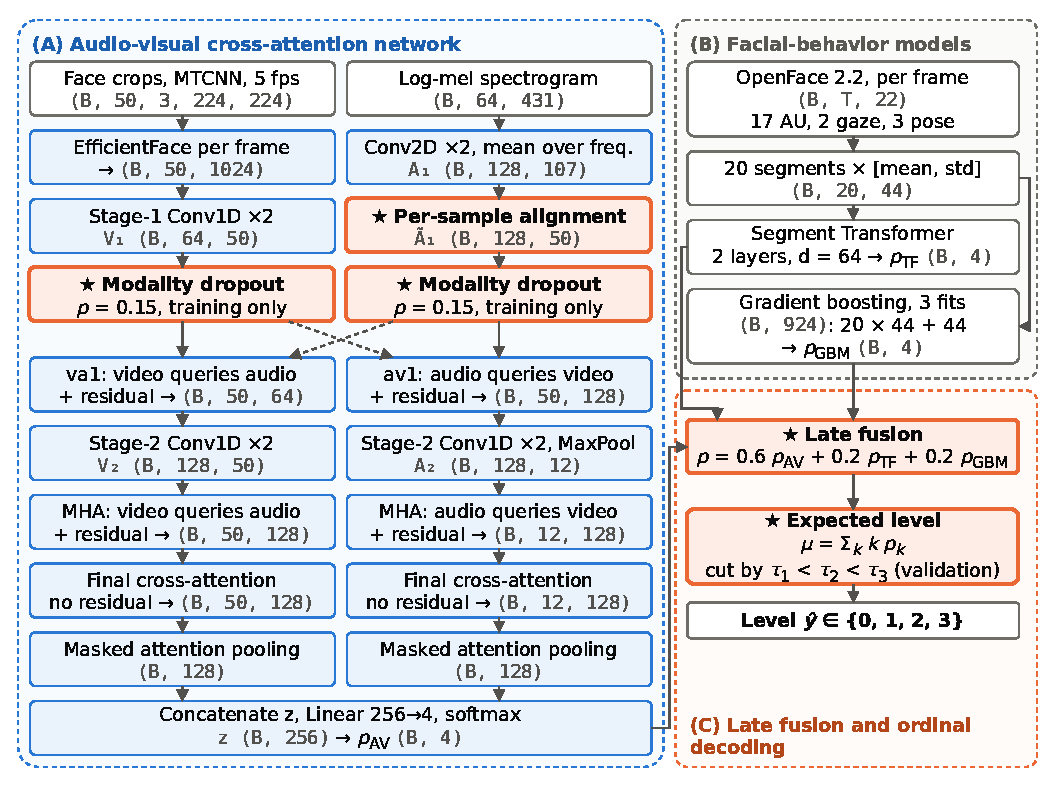
\includegraphics[width=\textwidth]{Fig2}
\caption{Proposed \ournet{} architecture in detail. Token shapes (length $\times$ width) are traced from a forward pass of the trained configuration. (A) Audio tokens are pooled onto the 50-step visual clock of the same clip before the first cross-attention exchange; after the second convolutional stage the audio stream has 12 tokens and the video stream 50; every attention block is cross-modal, and the final pair has no residual connection. (B) Two models on segment statistics of the per-frame OpenFace descriptor. (C) The three class-probability vectors are averaged with fixed weights, reduced to an expected level, and cut by thresholds fitted on the validation split. Blocks marked with a star are the components evaluated in Section~\ref{sec:results}; dashed arrows show the keys and values that each stream takes from the other in the first exchange}
\label{fig:arch}
\end{figure*}

\subsection{Audio-visual cross-attention network}\label{sec:method_av}

We pick the intermediate cross-attention fusion of AVT-CA \citep{venkatraman2025avtca} because in this fusion each modality attends to the other at three stages of the network, which uses multi-head attention with $h = 8$ heads throughout.

\subsubsection{Audio encoder}\label{sec:audio}

The audio track is resampled to 22.05\,kHz and converted to a 64-bin log-mel spectrogram $\mathbf{X}_a \in \mathbb{R}^{64 \times 431}$ for a 10\,s clip. Two convolution blocks ($3 \times 3$ convolution, batch normalization, ReLU, $2 \times 2$ max pooling) with 64 and 128 channels operate over frequency and time, and the frequency axis is averaged, which gives the first-stage audio tokens $\mathbf{A}_1 \in \mathbb{R}^{128 \times 107}$.

\subsubsection{Visual encoder}\label{sec:visual}

Each clip is sampled at 5 frames per second, which gives up to 50 face crops of $224 \times 224$ pixels detected with MTCNN \citep{zhang2016mtcnn}. An EfficientFace backbone \citep{zhao2021efficientface}, initialized from weights trained for facial expression recognition on AffectNet \citep{mollahosseini2019affectnet}, maps each frame to a 1024-dimensional embedding, and two one-dimensional convolution blocks (kernel size 3, batch normalization, ReLU; 1024$\to$64$\to$64) over the stacked embeddings give the first-stage visual tokens $\mathbf{V}_1 \in \mathbb{R}^{64 \times T_v}$ with $T_v \le 50$.

\subsubsection{Per-sample temporal alignment}\label{sec:align}

Each audio token should describe the same span of the clip as one visual token before the two streams exchange information; without this step, the 107 audio steps of a full clip describe it at twice the temporal resolution of its 50 visual tokens. We therefore pool the $L_a$ valid audio steps of every sample onto its $T_v$ valid visual tokens by adaptive average pooling over windows of nearly equal width (Online Resource~1, Section~S3), which gives the aligned tokens $\tilde{\mathbf{A}}_1 \in \mathbb{R}^{128 \times T_v}$. Padding steps are excluded before pooling and masked afterwards, so the alignment holds for clips of any length.

\subsubsection{Cross-attention fusion}\label{sec:xattn}

Let $\mathrm{MHA}(X_q, X_k)$ be multi-head scaled dot-product attention \citep{vaswani2017attention} with $X_q$ supplying the queries and $X_k$ the keys and values. In cross-attention, the queries and the keys come from different streams, and the two directions with residual connections are
\begin{align}
\tilde{X}_a &= X_a + \mathrm{MHA}(X_a, X_v) \label{eq:xattn_a}\\
\tilde{X}_v &= X_v + \mathrm{MHA}(X_v, X_a) \label{eq:xattn_v}
\end{align}
Here, $\tilde{X}_a$ and $\tilde{X}_v$ are the streams after the exchange; the attention matrix has shape $T_a \times T_v$, so the two lengths do not have to match. The network performs three such exchanges (Fig.~\ref{fig:arch}). In the first, $\tilde{\mathbf{A}}_1$ and $\mathbf{V}_1$ attend to each other through pre-normalized cross-attention blocks with a feed-forward sub-layer. A second convolutional stage then brings the audio tokens to $\mathbf{A}_2 \in \mathbb{R}^{128 \times 12}$ and the visual tokens to $\mathbf{V}_2 \in \mathbb{R}^{128 \times 50}$, and the second exchange lets them attend to each other with plain multi-head attention. The third exchange replaces each stream by its attention over the other, so that each stream ends as a summary of the other weighted by its own tokens. Each stream is reduced over time to a 128-dimensional vector by masked attention pooling, the two vectors are concatenated into the audio-visual summary $\mathbf{z} \in \mathbb{R}^{256}$, and a linear layer maps $\mathbf{z}$ to the four class probabilities $p_{\mathrm{AV}}$. The layer-by-layer configuration is given in Online Resource~1, Section~S3.

\subsubsection{Modality dropout and training objective}\label{sec:dropout}

To prevent the network from relying on one stream, during training we set the entire token sequence of each modality to zero with probability $p = 0.15$ per sample, independently for audio and video, where the first exchange begins; this also makes the inference-time modality ablation of Section~\ref{sec:abl_modality} a condition seen in training. The network is trained with the ordinal objective of Section~\ref{sec:method} with label smoothing of 0.1 and $\lambda = 0.15$, so that probability mass placed three levels from the true level costs more than mass placed one level away.

\subsection{Facial-behavior models}\label{sec:method_beh}

The second block predicts the engagement level from explicit OpenFace descriptors of the same clip, which the best EngageNet baseline uses \citep{singh2023engagenet} and on which gradient boosting has worked well in earlier engagement studies \citep{das2025optimizing,wang2026shap}.

\subsubsection{Segment statistics}\label{sec:segstats}

OpenFace 2.2 \citep{baltrusaitis2018openface} gives, per frame, 17 action-unit intensities, two gaze angles and three head-pose rotations, a 22-channel series. Following the best EngageNet baseline \citep{singh2023engagenet}, the series is divided into $S = 20$ equal segments, each described by the mean and standard deviation of every channel, a $20 \times 44$ token sequence $\mathbf{S}$.

\subsubsection{Gradient-boosting model}\label{sec:gbm}

The 20 tokens are flattened and extended with the clip-level mean and standard deviation of each channel, a 924-dimensional vector, on which a histogram gradient-boosting classifier \citep{pedregosa2011sklearn} with at most 15 leaves per tree is trained; three fits (learning rates 0.05, 0.03 and 0.05; 300, 600 and 300 iterations) are averaged to give $p_{\mathrm{GBM}}$.

\subsubsection{Segment-Transformer model}\label{sec:segtf}

A pre-norm Transformer encoder \citep{vaswani2017attention} with a class token and learned positional embeddings reads the 20 tokens of $\mathbf{S}$ and outputs $p_{\mathrm{TF}}$. It is trained with the same ordinal objective, AdamW with a warm-up cosine schedule, and random dropout of segment tokens; its configuration (two layers, width 64, eight heads, feed-forward width 128, learning rate $10^{-3}$) was selected from eight candidates by validation accuracy.

\subsection{Late fusion and ordinal decoding}\label{sec:method_fusion}

The third block combines the class-probability vectors of the three models by a weighted average, which is calculated as,
\begin{equation}
p = w_{\mathrm{AV}}\, p_{\mathrm{AV}} + w_{\mathrm{TF}}\, p_{\mathrm{TF}} + w_{\mathrm{GBM}}\, p_{\mathrm{GBM}} \label{eq:late}
\end{equation}
Here, $p_{\mathrm{AV}}$, $p_{\mathrm{TF}}$ and $p_{\mathrm{GBM}}$ are the class-probability vectors of the audio-visual network, the segment Transformer and the gradient-boosting model. The weights $(w_{\mathrm{AV}}, w_{\mathrm{TF}}, w_{\mathrm{GBM}})$ are fixed to $(0.6, 0.2, 0.2)$ for every seed. A grid search on the validation split selected this setting for seven of the eight networks we fused with the two behavior models (three seeds of the audio-visual network, three of the behavior-branch network of Section~\ref{sec:abl_branch} and two of its text variant). Fusing at the probability level keeps the three models independent, and Section~\ref{sec:res_sota} shows that many clips misclassified by the network are classified correctly by a behavior model. The fused vector $p$ is reduced to the expected level and cut by three thresholds fitted on the validation split only by a coordinate search and applied unchanged to the test split. For the network alone we compare four decoders: argmax, argmax after a per-class logit bias fitted on validation, expected-level thresholds fitted on a grid, and refined expected-level thresholds obtained by a local search; the search settings are given in Online Resource~1, Section~S1.

\section{Experiments}\label{sec:exp}

\subsection{Dataset}\label{sec:dataset}

We evaluate \ournet{} on EngageNet \citep{singh2023engagenet}, the online-learning engagement dataset with the largest number of participants, recorded with the participants' own webcams at sites such as computer labs and dorm rooms, so that some clips contain background noise. The recordings are divided into 11,311 ten-second clips (31\,h) of 127 participants. In all experiments, we use the official subject-independent split, which assigns 90, 11 and 26 participants to training, validation and test (7,983, 1,071 and 2,257 clips). We exclude the 105 clips that the dataset labels as ``subject not present'' (104 training clips and 1 test clip), since they carry no engagement level. Online Resource~1, Table~S8 shows the clips per level and split. The \emph{highly engaged} level accounts for 50.27\% of the test clips, so a constant majority-class predictor scores 50.27\% top-1 accuracy and 16.73 macro-F1, the reference for every result in this paper.


\subsection{Compared methods}\label{sec:baselines}

We compare \ournet{} with the six baselines released with EngageNet \citep{singh2023engagenet}, to our knowledge the only published results on the official test split: an LSTM, a CNN-LSTM, a temporal convolutional network (TCN) and a Transformer encoder on OpenFace gaze, head-pose and action-unit features summarized over time windows (98 values per window; the Transformer reads 20 equal windows, the tokenization our segment statistics follow), the same Transformer on MARLIN video features, and a fusion of the two feature sets. We take their test accuracies from the EngageNet paper and do not retrain them; the majority-class predictor is the second reference.

\subsection{Implementation details}\label{sec:impl}

We trained the audio-visual network, the gradient-boosting model and the segment Transformer separately; the configuration of each is listed in Online Resource~1, Table~S5. All clips are processed identically across the three splits: face frames are sampled at 5 frames per second, detected with MTCNN \citep{zhang2016mtcnn} and cropped to $224 \times 224$ pixels (a clip with more than 50 frames is subsampled uniformly to 50, a shorter one is padded with masked frames), the audio track is converted to the log-mel spectrogram of Section~\ref{sec:audio}, and the facial-behavior series are collected with OpenFace 2.2 \citep{baltrusaitis2018openface}, which detects a face in 98.2\% of the frames. Before the reported fine-tuning, the network was trained on EngageNet in three stages from the AffectNet initialization of the visual backbone (Online Resource~1, Section~S4). All reported networks are fine-tuned from the resulting checkpoint with three random seeds, about 32 minutes per run on one NVIDIA RTX 3090 GPU; the two behavior models were trained on the training split only. The networks were implemented in PyTorch 2.5 and the gradient-boosting model in scikit-learn \citep{pedregosa2011sklearn}. The test split is used only for the final evaluation: the kept checkpoint of each run, the size of the segment Transformer, the fusion weights and the decoding thresholds are all chosen on the validation split, and each reported test result is computed once. Generative AI was used in preparing this study as described in the Statements and Declarations; it did not produce data, and every reported number was computed by the authors' code from the trained models.


\section{Results and discussion}\label{sec:results}

We report four metrics on the 2,256 test clips: top-1 accuracy, adjacent accuracy (the fraction of clips predicted within one level of the truth), the mean absolute error (MAE) in levels, and macro-F1, which cannot be raised by predicting the majority level; their definitions are given in Online Resource~1, Section~S2. Unless stated otherwise, a result is the mean over three seeds, the network alone is decoded with its refined expected-level thresholds, and $\pm$ values are standard deviations over seeds.

\subsection{Comparison with published baselines}\label{sec:res_sota}

\begin{table*}[t]
\tablebodyfont
\caption{Comparison of \ournet{} with published results on EngageNet. G, HP, AU: OpenFace gaze, head-pose and action-unit features; rPPG: physiological signals estimated from the video. Only the test-split rows are directly comparable}\label{tab:related}
\begin{tabular*}{\textwidth}{@{\extracolsep\fill}llllr}
\toprule
Work & Model & Input & Split & Top-1 (\%)\\
\midrule
\citet{singh2023engagenet} & LSTM & G+HP+AU & Test & 61.84\\
 & CNN-LSTM & G+HP+AU & Test & 65.16\\
 & TCN & G+HP+AU & Test & 65.60\\
 & Transformer & G+HP+AU & Test & 67.61\\
 & Transformer & MARLIN & Test & 65.20\\
 & Transformer & G+HP+AU, MARLIN & Test & 66.50\\
\citet{vedernikov2024tcct} & TCCT-Net & Head pose & Validation & 68.91\\
\citet{abedi2024stgcn} & Ordinal ST-GCN & Facial landmarks & Validation & 71.24\\
\citet{augusma2026vemd} & VE-MD & Video & Validation & 68.98\\
\citet{vedernikov2026priornet} & PriorNet & Face video & Validation & 73.58\\
\citet{qin2026glpfusion} & GLP-fusion & Face, key points, rPPG & Own split$^{a}$ & 63.78\\
\midrule
Ours & \ournet & Face, audio, G+HP+AU & Test & 70.29\\
\botrule
\end{tabular*}
\begin{tablenotes}
\item $^{a}$EmotiW 2023 data \citep{dhall2023emotiw}, re-partitioned by the authors
\end{tablenotes}
\end{table*}


Table~\ref{tab:related} lists the published results on EngageNet together with \ournet{} and its components; the six baselines read OpenFace features, MARLIN video features \citep{cai2023marlin}, or both. The baselines are reported on the official test split; the later methods report validation accuracy, on which the same baseline model scores 1.5--5.2 points higher, or use a split of their own, so their rows are listed for context and are not compared directly. \ournet{} achieves the highest top-1 accuracy on the test split, 70.29 $\pm$ 0.14\%, against 67.61\% for the best baseline. The audio-visual network alone reaches 66.27 $\pm$ 0.45\%, above four of the six baselines but below the best one. The gradient-boosting model and the segment Transformer, which read only 22 of the 49 per-frame OpenFace channels behind the 98 features of the best baseline, reach the same range as the network (66.27\% and 66.99\%). The fusion gain comes from errors that the models do not share: the network and the gradient-boosting model are each wrong on about 34\% of the test clips, but both are wrong on only about 22\%. Tested on the same clips, \ournet{} is more accurate than each of its members for every seed (exact McNemar test, $p \le 0.006$; Online Resource~1, Table~S11).

Two points qualify this comparison. It is not like-for-like, since \ournet{} averages three models and fits its thresholds on the validation split, whereas each baseline is a single model decoded from its softmax output; and the best baseline is not a strong bound for its own features, since a gradient-boosting model on the same 98 OpenFace features reaches 68.13\% with argmax decoding and 68.88\% with expected-level thresholds (Section~\ref{sec:abl_fusion}), so part of the margin comes from the learner and the decoding rule rather than from the audio-visual network.

\subsection{Per-seed and per-level results}\label{sec:res_seed}

Table~\ref{tab:seeds} reports every model per seed with the four metrics. \ournet{} has the highest top-1 accuracy and macro-F1 and the lowest mean absolute error of all trained models, and the smallest seed spread of the seeded models; only the adjacent accuracy of the audio-visual network is slightly higher. For every model that sees the face, most errors are one-level errors: its adjacent accuracy is more than 20 points above its top-1 accuracy.

\begin{table*}[t]
\tablebodyfont
\caption{Test results per seed (top-1, \%) and mean over three seeds. The one-input network rows are the ablation of Section~\ref{sec:abl_modality}; the gradient-boosting model is one averaged model}\label{tab:seeds}
\begin{tabular*}{\textwidth}{@{\extracolsep\fill}lccccccc}
\toprule
Model & Seed 1 & Seed 2 & Seed 3 & Top-1 & Adj. & MAE & Macro-F1\\
\midrule
Majority-class predictor & 50.27 & 50.27 & 50.27 & 50.27 & 68.84 & 1.012 & 16.73\\
Network, audio only & 46.59 & 50.27 & 50.27 & 49.04 $\pm$ 2.12 & 69.27 & 1.004 & 17.35\\
Network, video only & 65.60 & 65.56 & 64.67 & 65.28 $\pm$ 0.53 & 90.77 & 0.459 & 51.29\\
Audio-visual network & 65.78 & 66.36 & 66.67 & 66.27 $\pm$ 0.45 & \textbf{91.55} & 0.440 & 52.31\\
Gradient boosting & 66.27 & 66.27 & 66.27 & 66.27 & 89.01 & 0.476 & 50.04\\
Segment Transformer & 67.02 & 67.91 & 66.05 & 66.99 $\pm$ 0.93 & 87.90 & 0.487 & 49.45\\
\textbf{\ournet} & 70.17 & 70.26 & 70.43 & \textbf{70.29 $\pm$ 0.14} & 91.06 & \textbf{0.401} & \textbf{53.95}\\
\botrule
\end{tabular*}
\end{table*}

Online Resource~1, Table~S6 reports precision, recall and F1 per level. The two extreme levels are recognized well by every model, and the two middle levels are not. The three models fail on the middle levels in different ways: the gradient-boosting model almost never predicts \emph{barely engaged} (recall 1.6\%) but has the highest recall on \emph{engaged} (59.4\%), whereas the network has the highest recall on \emph{barely engaged} (17.8\%). Fusion raises the F1 of \emph{engaged} from 28.8 to 39.8 and of \emph{highly engaged} from 80.3 to 85.1, and lowers the F1 of \emph{barely engaged} from 22.3 to 15.4.


\subsection{Effect of the decoding rule}\label{sec:res_decoder}

Table~\ref{tab:decoder} isolates the decoding rule of Section~\ref{sec:method} on the audio-visual network. Replacing argmax with expected-level thresholds adds 1.99 points of top-1 accuracy for the network and 1.80 points for its video-only condition, with no change to the weights and no test data used in the fit. This gain is larger than the effect of any single training change in the sweep of Online Resource~1, Table~S2, and larger than the gap between the two best published baselines (1.11 points), which decode a softmax output with argmax.

\begin{table}[t]
\caption{Effect of the decoding rule on the same trained weights (test top-1, \%, three seeds). Thresholds: expected-level thresholds fitted on validation on a grid; refined: the same after a local search; differences computed before rounding}\label{tab:decoder}
\begin{tabular*}{\columnwidth}{@{\extracolsep\fill}lcc}
\toprule
Decoder & Audio + video & Video only\\
\midrule
Argmax & 64.27 $\pm$ 0.22 & 63.48 $\pm$ 0.35\\
Fitted logit bias & 65.06 $\pm$ 0.37 & 63.83 $\pm$ 0.45\\
Thresholds & \textbf{66.34 $\pm$ 0.50} & 65.26 $\pm$ 0.40\\
Refined thresholds & 66.27 $\pm$ 0.45 & \textbf{65.28 $\pm$ 0.53}\\
\midrule
Refined $-$ argmax & +1.99 & +1.80\\
\botrule
\end{tabular*}
\end{table}

\subsection{Ablation studies}\label{sec:ablation}

We performed five ablation studies on the EngageNet test split; four are reported here and the fifth, a sweep of fourteen fine-tuning runs of the network from one checkpoint that vary its training settings, in Online Resource~1, Section~S5, where no single change raises accuracy beyond the seed spread. Three seeds of one configuration give a standard deviation of 0.45 points of top-1 accuracy, and the binomial 95\% confidence interval on 2,256 test clips is about $\pm$1.95 points, so we treat a difference in three-seed means below about one point as within noise and rely on the consistency of sign across matched models for smaller effects.

\subsubsection{Contribution of each modality}\label{sec:abl_modality}

This ablation asks whether the audio track contributes to a network that was trained with it, and by how much. Instead of training separate unimodal models, we kept the trained weights unchanged and set the token sequence of one modality to zero at inference, the same operation as modality dropout, for the nine fine-tuned networks of this work: three seeds each of the audio-visual network and of the two behavior-branch variants of Section~\ref{sec:abl_branch}. Audio alone scores at or below the majority-class predictor in all nine networks (mean 48.60\%), so audio by itself does not predict engagement on this dataset. Adding audio to video raises top-1 accuracy in seven of the nine networks, leaves it unchanged in one and lowers it by 0.13 points in one, by 0.74 points on average (from 65.41\% to 66.15\%; Online Resource~1, Table~S9). Only one difference (1.99 points) remains significant after adjustment for multiple testing (exact McNemar test; Online Resource~1, Table~S12), and the nine networks share one warm start, so the evidence is the consistent sign rather than any single network; in an earlier sweep, ten further networks from the same warm start show the same sign in nine. Macro-F1 is higher with audio in six of the nine networks.


\subsubsection{Behavior branch inside the network}\label{sec:abl_branch}

This ablation asks whether the two separate behavior models are necessary, or whether the network can absorb the same descriptors through a branch of its own. We attached a behavior branch to the same warm start as the audio-visual network: a one-dimensional convolution and a bidirectional GRU encode the OpenFace series on the 50-step visual clock, the summary $\mathbf{z}$ attends over these tokens, and the classifier reads $\mathbf{z}$, the attended vector and a projection of the clip-level descriptor mean. The new classifier columns were initialized to zero, so that at the start of fine-tuning the model is exactly the audio-visual network, and the branch was fine-tuned with the same schedule and seeds. A second variant adds a text rendering of the same action-unit series as a further input. Neither variant changes any metric by more than a fraction of the seed standard deviation (top-1 66.08 $\pm$ 0.59\% and 66.12 $\pm$ 0.59\% against 66.27 $\pm$ 0.45\%; Online Resource~1, Table~S7). The same descriptors raise accuracy when they are used through the separate models of block B: with a behavior-branch network in place of the audio-visual network as the neural member of the fusion, the fused accuracy is 69.9--70.3\% over three seeds. The descriptors are therefore informative, and the per-frame recurrent branch does not extract what the segment statistics provide.


\subsubsection{Fusion weights}\label{sec:abl_fusion}

This ablation asks how much the result depends on the particular fusion weights. We evaluated the fusion of block C under different weight rules, keeping all three models unchanged (Online Resource~1, Table~S10). Every weight rule in Table~S10 that includes the gradient-boosting model gives between 67.4\% and 70.5\% on every seed, and equal weights, which involve no selection, give 69.28 $\pm$ 0.23\%. With the gradient-boosting model alone, any network weight from 0.5 to 0.7 gives 69.95--70.07\%, and accuracy drops once the network dominates the average (Online Resource~1, Fig.~S1). Fusing the network with the segment Transformer alone is unstable across seeds (68.69 $\pm$ 2.08\% with validation-selected weights), because the validation accuracy of the Transformer does not follow its test accuracy closely; adding the gradient-boosting model reduces the standard deviation to 0.14 points. Finally, with the full 98-dimensional OpenFace descriptor of the best baseline, the gradient-boosting model alone reaches 68.88\% (68.13\% with argmax decoding), above the published Transformer on the same features, but the three-way fusion does not improve (69.15 $\pm$ 0.83\% over the eight networks of Section~\ref{sec:method_fusion}, with validation-selected weights).


\subsubsection{Number of segments}\label{sec:abl_segments}

This ablation asks whether the 20-segment tokenization inherited from the strongest baseline is the right granularity for the behavior models. We re-ran the gradient-boosting model for $S \in \{1, 5, 10, 20, 40\}$ segments, keeping the segment Transformer at $S = 20$ (Online Resource~1, Table~S1). The number of segments changes its top-1 accuracy by about one point at most, and even $S = 1$, which keeps only the clip-level mean and standard deviation, reaches 67.29\%; every fused setting stays between 68.8\% and 70.6\%, so the result of \ournet{} does not depend on the choice of $S = 20$, which we fixed before this test to match the baseline.

\subsection{Computational cost}\label{sec:res_cost}

Online Resource~1, Table~S3 reports the size and inference cost of each component on real test clips with batch size 1. The audio-visual network has 2.38\,M parameters and needs 16.0\,GFLOPs per 10\,s clip, almost all of it in the frame encoder; it processes a clip in 21.5\,ms on one RTX 3090 GPU and in 271\,ms on eight CPU threads, and the two behavior models are small. The most expensive step is the OpenFace extraction that feeds block B, a median of 11.3\,s per clip on one CPU thread, about the duration of the clip, so real-time use needs OpenFace on several threads or a faster extractor.

\subsection{Error analysis}\label{sec:res_errors}

Fig.~\ref{fig:confusion} presents the row-normalized test confusion matrices of the audio-visual network and of \ournet, pooled over the three seeds. The network recognizes the two extreme levels in 77\% and 87\% of cases, but \emph{barely engaged} and \emph{engaged} in only 18\% and 26\%; three quarters of its errors (74.9\%) are off by one level, and two thirds (67.4\%) are on the two middle levels, which make up 29.5\% of the test set. \ournet{} shifts recall toward the upper half of the scale, raising it on \emph{highly engaged} from 87\% to 94\% and on \emph{engaged} from 26\% to 38\% while lowering it on \emph{not engaged} from 77\% to 73\% and on \emph{barely engaged} from 18\% to 11\%, so an even larger share of its errors (71.8\%) is on the two middle levels.

\begin{figure}[t]
\centering
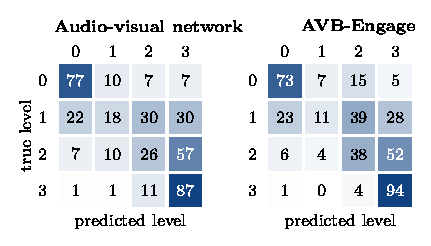
\includegraphics[width=\columnwidth]{Fig3}
\caption{Row-normalized test confusion matrices (\%) of the audio-visual network (left) and \ournet{} (right), pooled over three seeds. Levels 0--3: not, barely, engaged, highly engaged}
\label{fig:confusion}
\end{figure}

We see two reasons for this behavior. First, the two middle levels describe a difference of degree in similar visible behavior: a student who looks at the screen with a neutral face may be labeled \emph{barely engaged} or \emph{engaged}, and a ten-second clip of a student watching an educational video contains no response to an instructor that would separate the two. Second, the label prior differs between the splits (12.3\% \emph{not engaged} clips in validation against 20.3\% in test), so thresholds fitted on validation are not the best thresholds for test; for the seed-1 network, thresholds fitted on the test split itself would give 67.82\% instead of the 65.69\% of the same search on validation, an upper bound rather than a method. Merging the two middle levels in the output of one trained network (seed 3, argmax decoding), without retraining, raises top-1 accuracy from 64.27\% to 70.70\% against an unchanged majority-class accuracy (Online Resource~1, Table~S4), which locates the errors between these two levels.

\subsection{Challenges and future directions}\label{sec:limitations}

The results mark out three challenges for the next studies. \emph{Datasets.} The evaluation uses a single dataset, whose participants watch short educational videos and rarely speak, so the audio contribution measured here (0.74 points) is likely a lower bound for settings in which students speak and listen in turn; recordings of live online classes with per-participant audio are the natural next evaluation. \emph{Middle levels.} \emph{Barely engaged} is recognized in at most 18\% of cases by any model on average over seeds, and in 2--5\% by the two behavior models, so the remaining errors lie in the two middle levels rather than in any one modality. Since the labels are themselves human judgements, a survey in which raters with teaching experience label a stratified sample of test clips will show whether these levels are also hard for people. \emph{Design choices and cost.} The temporal alignment and the modality dropout were adopted from the emotion-recognition setting and kept fixed; matched runs without them will quantify their individual effect. Part of the margin over the published baselines comes from the decoding rule and the learner rather than from the network (Section~\ref{sec:res_sota}), and both steps apply to any classifier. OpenFace extraction takes about as long as the clip on one CPU thread, so a lighter descriptor extractor would make \ournet{} usable in real time.

\section{Conclusion}\label{sec:conclusion}

We presented \ournet, which combines an audio-visual cross-attention network with two models on segment statistics of OpenFace descriptors and decodes the four ordered engagement levels through the expected level. Our experiments on the official EngageNet test split over three training seeds show that \ournet{} exceeds the published baselines, with 70.29\% against 67.61\%, and that most of this gain comes from two steps that do not depend on the network architecture: decoding through the expected level, and averaging models that make different errors. The audio track has no standalone signal on this dataset, but it raised accuracy in seven of nine networks when fused with video, and the facial-behavior descriptors helped when they were summarized by segment statistics in separate models, not when they were learned by a recurrent branch inside the network. One shortcoming of this work is that it uses a single dataset in which students rarely speak. Evaluating the model on live online classes with per-participant audio, and a human labeling study of the two middle levels, are the directions of our future work.

\backmatter

\bmhead{Supplementary information}
The supplementary file, Online Resource 1 (ESM\_1.pdf), gives the decoding rules and threshold search, the training objective, metrics, alignment, cross-attention blocks, training procedure and configuration, and further ablation, cost, label-granularity, per-level, behavior-branch, dataset, modality, fusion-weight and significance results.

% \bmhead{Acknowledgements} -- optional in the template; add here if the authors wish to acknowledge anyone.

\section*{Statements and Declarations}

\bmhead{Funding}
The authors did not receive support from any organization for the submitted work.

\bmhead{Competing interests}
The authors have no relevant financial or non-financial interests to disclose.

\bmhead{Ethics approval and consent to participate}
No new data were collected for this study. It uses the EngageNet dataset, obtained from its authors on request, whose participants consented to the use of their data when it was recorded \citep{singh2023engagenet}.

\bmhead{Data availability}
The EngageNet dataset is available from its authors on request \citep{singh2023engagenet}. The per-clip predictions of this study are available from the corresponding author on reasonable request.

\bmhead{Materials availability}
Not applicable.

\bmhead{Code availability}
The code is publicly available at \url{https://github.com/YuvrajGupta1808/AVTCA-Research}.

\bmhead{Author contributions}
Yuvraj Gupta: Conceptualization, Methodology, Software, Validation, Formal analysis, Investigation, Data curation, Visualization, Writing -- original draft. Sanchita Ghose: Conceptualization, Supervision, Writing -- review and editing. Both authors read and approved the final manuscript.

\bmhead{Use of generative AI}
The authors used generative AI tools, following their specifications, to help write and debug the experiment and analysis code, check bibliographic metadata, and draft and edit text. The authors designed and ran all experiments, reviewed and revised all content, and take full responsibility for the article.

\bibliography{references}% formatted by sn-basic.bst (selected by the sn-basic class option)

\end{document}
